\documentclass[thesis.tex]{subfile}

\chapter{Implementation}
\label{ch:implementation}

We discuss our implementation of time-tiling in detail (Section~\ref{sec:time-tiling}).
The latter extends the former, while depending crucially on an initial skewing transformation.
We examine the safeguards necessary to prevent errors caused by improper skewing.
Finally, we consider the implications on sparse loops, one of Devito's raisons d'\^etre.


\section{Skewing and Devito transformations}
\label{sec:time-tiling}

As outlined in Section~\ref{sec:bg-time-tiling}, we implement time-tiling in two stages: skewing in the DSE (Section~\ref{sec:dse}), and tiling in the DLE (Section~\ref{sec:dle}).

\section{Skewing}
\label{sec:skewing}
In our implementation, inner loops are skewed by a factor of time, and the loop bounds skewed by the same factor, negated.
This ensures that all accesses refer to the same data as before the transformation, making it valid.
Note that skewing \emph{does not} change the execution order of the loops.

\paragraph{Common sub-expression elimination}
As skewing is merely a substitution of indices and loop bounds, we do not expect to change the expressions.
Since arithmetic on floats is generally non-commutative, we especially wish to avoid changing the structure of expressions, to simplify testing of the code.
In particular, we ensure than skewing is performed \emph{before} CSE occurs, to avoid expansion during skewing.


\section{Time-tiling}
We then change the tiling algorithm to use the \texttt{min} scheme, rather than remainder loops.
As we noted in the previous section, this will not change the execution order: we now have skewed tiles on a skewed iteration space (Figure~\ref{fig:skewed-loops-skewed-space}).
We now need to `straighten' the tiles by aligning the loop bounds.

% TODO: vague
\begin{figure}[!ht]
	\centering
	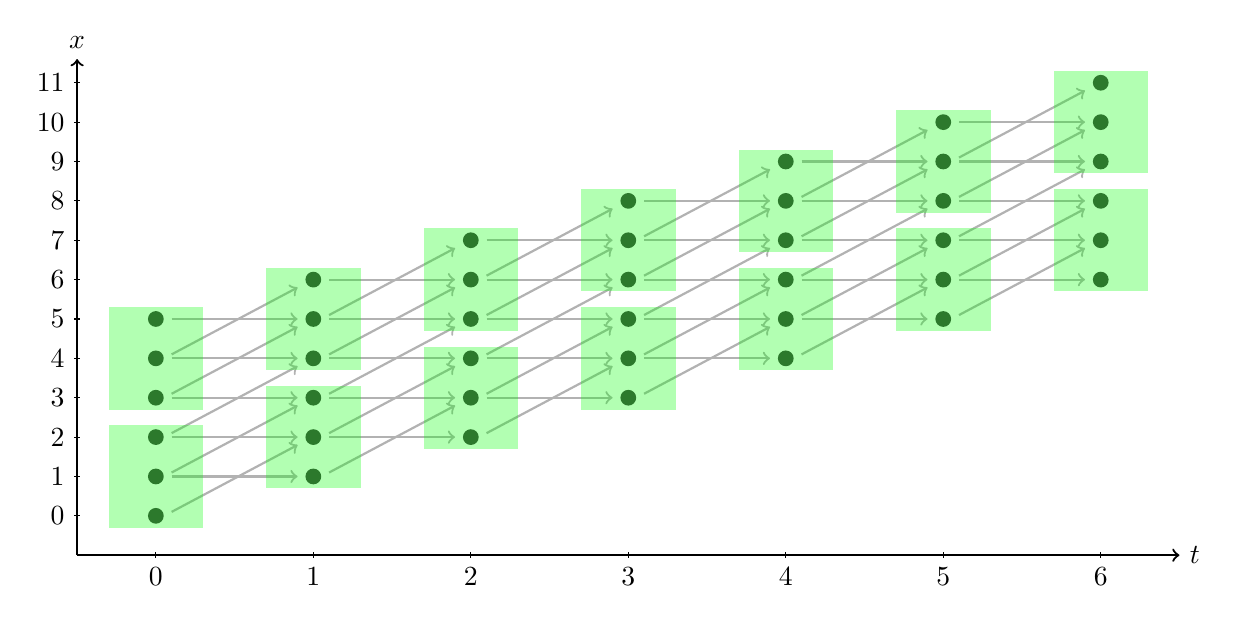
\begin{tikzpicture}
	\draw[thick,->] (-1,-.5) -- (13,-.5) node[right]{$t$};
	\draw[thick,->] (-1,-.5) -- (-1,5.8) node[above]{$x$};
	
	\foreach \t in {0,1,2,3,4,5,6}
	\foreach \x in {0,1,2,3,4,5}
	\fill[darkgray] (\t*2,\x/2+\t/2) circle (0.1);
	
	\foreach \t in {0,1,2,3,4,5}
	\foreach \x in {1,2,3,4,5}
	\draw[thick,->,gray!60] (\t*2+.2,\x/2+\t/2) -- (\t*2+1.8,\x/2+\t/2);
	
	\foreach \t in {0,1,2,3,4,5}
	\foreach \x in {0,1,2,3,4}
	\draw[thick,->,gray!60] (\t*2+.2,\x/2+\t/2+.05) -- (\t*2+1.8,\x/2+\t/2+.9);
	
	\foreach \t in {0,1,2,3,4,5,6}
	\foreach \x in {0,3}
	\fill[green,opacity=0.3] (\t*2-.6,\x/2+\t/2-.15) rectangle (\t*2+.6,\x/2+\t/2+1.15);
	
	\foreach \t in {0,1,2,3,4,5,6}
	\draw (\t*2,1pt-.5cm) -- (\t*2,-1pt-.5cm) node[anchor=north] {$\t$};
	\foreach \x in {0,1,2,3,4,5,6,7,8,9,10,11}
	\draw (1pt-1cm,\x/2) -- (-1pt-1cm,\x/2) node[anchor=east] {$\x$};
	\end{tikzpicture}
	\caption{Skewed tiles on a skewed iteration space. Dependencies between blocks have not changed, and interchange is not valid.}
	\label{fig:skewed-loops-skewed-space}
\end{figure}

Having straightened the tiles (as in Figure~\ref{fig:dependence-skew}),

% Parallelism troubles leading to the Visitor

\section{Remaining work}
The implementation work that remains can be divided into several tasks:

\begin{description}
	\item[Straightening of tiles] (end Feb.) This will make the interchange valid, enabling time-tiling. There are a number of concerns:
	\begin{itemize}
		\item The actual straightening, involving some reasoning about loop bounds, use of \texttt{max} -- trivial
		\item Modification to tile the time loop, possibly by incorporating the \texttt{blockshape} parameter -- moderate difficulty due to test cases
		\item Removal of `empty' blocks -- trivial; does not affect correctness but might produce speedup\footnote{CLooG does it, but one has difficulty imagining that there will indeed be a noticeable speedup}
		\item Making this work with time buffering -- some reasoning about skewing factor required
		\item Test cases -- important; partially done
		\item Removal of test cases assuming a remainder loop structure.
		\item Verification that a given skewing factor is valid -- deferred
	\end{itemize}

	\item[Verification of skewing validity] This may be challenging.\footnote{It should be quite easy with knowledge of the data dependence vectors.} For the moment, skewing will work via manual input of skewing factors, hence shifting the responsibility of this onto the user. Clearly, this is not a viable strategy for code acceptance and usage, but it will (minimally) enable our evaluation.

	\item[DSE aggressive mode] Currently, no reason to suppose that this cannot work with \texttt{min}-bounded instead of remainder loops. Need to prove/disprove this, and make it work. Revert to remainder loops if necessary. In particular, we must examine the references made to certain variables.\footnote{Of particular interest are \texttt{blockshape} (the tile size) and dimension extents (e.g.~symbolic extent vs offsets).}

	\item[Sparse loop interpolation] Gather more context and understanding of the problem will be important for reasoning about how this affects time-tiling. Ideally, eventually a proof of what it does/why it does not.

	\item[Detection of when to apply skewing and calculation of the skewing factor] Whether time-tiling is an appropriate optimisation, for a given stencil. Entirely beyond the scope of this work.
\end{description}
